% Generated by scripts/build_pro_latex.py from manuscrito_final/manuscript.md; do not edit by hand.
\documentclass[10pt]{article}
\usepackage{sga_manuscrito}
\hypersetup{pdftitle={Predictive modeling of outcomes in salivary gland cancers using machine learning: simulated prospective validation with the RTOG 1008 trial},pdfauthor={Federico Lorenzo, Agustin Rosich, Jesica Lell, Sergio Aguiar, Valentina Ferreira, Karina Ochandorena, Eduardo Larrinaga, Natalia Gadea, Nicolas Larragueta, Aldo Quarneti}}
\runningtitle{Adding chemotherapy to RT in salivary cancer}
\manuscriptauthors{Federico Lorenzo\textsuperscript{1,2}, Agustin Rosich\textsuperscript{1,2}, Jesica Lell\textsuperscript{1,2}, Sergio Aguiar\textsuperscript{1}, Valentina Ferreira\textsuperscript{1}, Karina Ochandorena\textsuperscript{1,2}, Eduardo Larrinaga\textsuperscript{1}, Natalia Gadea\textsuperscript{1}, Nicolas Larragueta\textsuperscript{1}, Aldo Quarneti\textsuperscript{1}}
\manuscriptaffiliations{\textsuperscript{1}Radiotherapy, RT International Institute, Montevideo, Uruguay. \textsuperscript{2}Radiotherapy, Unidad Academica de Radioterapia, Montevideo, Uruguay, RT International Institute.}

\begin{document}

\maketitleblock{Predictive modeling of outcomes in salivary gland cancers using machine learning: simulated prospective validation with the RTOG 1008 trial}

\section{Abstract}

\subsection{Purpose}

Whether chemotherapy improves survival when added to radiotherapy in high-risk salivary gland cancer remains unresolved. We developed a falsifiable pre-results model predicting the average survival effect of chemotherapy in advanced T3/T4 disease for future comparison with RTOG 1008.

\subsection{Methods and Materials}

We analyzed a standardized Surveillance, Epidemiology, and End Results (SEER)-derived cohort of T3/T4 tumors with known N category and radiotherapy (RT). Overall survival was modeled with censoring. The prespecified estimand was the average treatment effect (ATE), expressed as the difference in restricted mean survival time (RMST) through 120 months for RT + chemotherapy versus RT only. Propensity-score weighting and a covariate-adjusted Cox model were used to address measured treatment-selection differences. Both potential outcomes were standardized to the same population, and the full analysis was repeated in 1,000 patient-level bootstrap samples. Internal performance was assessed by five-fold cross-validation.

\subsection{Results}

Of 4,657 source records, 954 met the eligibility criteria; 283 received RT + chemotherapy and 671 received RT only. Adjusted 10-year RMST was 64.8 months with RT + chemotherapy and 67.1 months with RT only. The ATE was −2.3 months (95\% bootstrap CI, −9.6 to +6.0; P=0.580). Adjusted absolute survival differences were −2.2 percentage points at both 5 and 10 years. Median follow-up by reverse Kaplan–Meier was 86 months. Mean cross-validated C-index was 0.641; inverse-probability-of-censoring-weighted Brier scores were 0.215 at 5 years and 0.188 at 10 years.

\subsection{Conclusions}

The model predicted no average overall-survival benefit from adding chemotherapy to radiotherapy in advanced T3/T4 disease. The estimate is consistent with the retrospective evidence against routine chemotherapy intensification and provides a pre-results prediction for prospective testing against RTOG 1008.

\FloatBarrier
\section{Introduction}

Surgery followed by risk-adapted postoperative radiotherapy is the established locoregional strategy for high-risk salivary gland malignancies [1–9], whereas the incremental value of chemotherapy remains unresolved [1,2,10]. Early institutional reports suggested a possible advantage from treatment intensification [11,12], but larger retrospective comparisons have not demonstrated a consistent survival benefit [13–21]. RTOG 1008 was designed to resolve this question by comparing postoperative radiotherapy alone with radiotherapy plus weekly cisplatin in resected high-risk disease [22–24].

The objective of this study was to predict whether chemotherapy produces a clinically relevant average survival gain when added to radiotherapy in advanced T3/T4 salivary gland cancer. We used censoring-aware causal survival methods and retained the RTOG 1008 sample size only as a secondary simulation benchmark.

\FloatBarrier
\section{Methods and Materials}

\subsection{Data source and implementable eligibility}

The source was a standardized extract from the National Cancer Institute SEER Program containing 4,657 records and 11 variables: grouped age, sex, ICD-O-3 histology, harmonized histology, harmonized T and N categories, binary radiotherapy and chemotherapy indicators, diagnosis-to-first-treatment delay, recoded cause of death, and survival months. We sequentially required T3/T4 disease, known N category, recorded radiotherapy, and nonmissing survival time.

This was an observational RTOG 1008-like analysis. Diagnosis was the available time origin, and treatment was classified from the registry indicators for radiotherapy and chemotherapy. Because SEER data are deidentified and publicly available, this analysis was exempt from institutional review board review.

\subsection{Treatment, endpoint, and estimand}

Treatment groups were labeled RT only and RT + chemotherapy. The registry did not specify the systemic agent or confirm concurrency.

The primary endpoint was overall survival. Any recorded death counted as an event; patients coded alive were censored at their observed last follow-up. Follow-up was administratively truncated at 120 months. A separate secondary cause-specific model counted salivary-gland cancer deaths as events and censored other causes.

Overall survival was the primary endpoint. The prespecified treatment-effect estimand was the ATE expressed as mean RMST with RT + chemotherapy minus mean RMST with RT only through 120 months. RMST does not replace overall survival; it summarizes the area under the overall-survival curve as average survival time within the 10-year horizon and expresses the treatment contrast directly in months without requiring proportional hazards. Secondary estimands were absolute adjusted survival differences at 60 and 120 months. Before examining results, a 6-month absolute RMST difference or a 5-percentage-point absolute survival difference was designated clinically relevant.

\subsection{Confounding adjustment, positivity, and balance}

Propensity scores were estimated by logistic regression from age, sex, T category, N category, and histology. Stabilized ATE weights were truncated at their first and 99th percentiles. Positivity was evaluated from treatment-specific propensity distributions and their 1st–99th percentile common support. Balance was assessed with standardized mean differences (SMDs), using |SMD| <0.10 as the diagnostic target.

We then fitted a weighted Cox proportional-hazards outcome model that also adjusted for all propensity covariates. This combined weighting and outcome adjustment was used as a doubly adjusted strategy against measured confounding. Marginal counterfactual survival curves were generated by setting treatment to each level for every patient and averaging predictions over the same 954-person population. RMST was obtained by integrating those marginal curves.

\subsection{Bootstrap and internal validation}

The nonparametric bootstrap resampled patients with replacement. Within every one of 1,000 iterations, the analytic sample, propensity model, stabilized and truncated weights, adjusted weighted Cox model, counterfactual survival curves, RMSTs, and treatment contrasts were recalculated. Percentile 95\% confidence intervals summarize sampling uncertainty. Two-sided P values for RMST and fixed-time survival differences were calculated with a normal approximation using the bootstrap standard error. The fraction of bootstrap estimates above zero was not interpreted as a clinical probability of benefit.

Five-fold internal cross-validation refitted preprocessing, propensity weights, and the outcome model within each training fold. Evaluation in held-out patients used Harrell's C-index, IPCW time-dependent Brier scores, and calibration error (mean predicted minus Kaplan–Meier observed risk) at 60 and 120 months. A gradient-boosting mortality classifier and its AUC were removed because they do not validate a censored survival model. Analyses were performed in Python 3.14 using lifelines 0.30, scikit-learn 1.9, pandas 2.3, NumPy 2.5, and SciPy 1.18, with a fixed random seed.

\subsection{Sensitivity and secondary analyses}

Prespecified sensitivity analyses excluded squamous carcinoma and restricted the cohort to histologies most comparable with RTOG 1008 that were identifiable in the extract: mucoepidermoid, adenocarcinoma, acinar cell, adenoid cystic, carcinoma NOS, and carcinoma ex pleomorphic adenoma. Descriptive histology-specific estimates were limited to groups with at least 80 patients and at least 15 patients per exposure; no subgroup p-values or post hoc benefit categories were used. An approximate E-value assessed sensitivity of the treatment hazard ratio to unmeasured confounding.

The full cohort remained primary. As an illustrative secondary analysis only, 1,000 samples of 252 patients were drawn and assigned 1:1. Potential RMST under both treatments was retained for each sampled patient, and standardized balance was recorded in every simulation.

\FloatBarrier
\section{Results}

\subsection{Cohort selection and observed treatment groups}

The cohort-selection summary (Supplementary Table S1) shows how the 4,657 source records were reduced to the 954 patients included in the primary analysis. Most exclusions resulted from disease outside T3/T4 (n=2,990); the subsequent steps excluded 276 patients with unknown N category and 437 without recorded radiotherapy, and no patient lacked a survival time.

The RT + chemotherapy group was younger, more frequently male, and had more T4 and node-positive disease, demonstrating substantial treatment-selection differences before adjustment (Table 1). Median diagnosis-to-first-treatment delay was 23 days (interquartile range [IQR], 0–47) with RT only and 26 days (IQR, 0–41) with RT + chemotherapy. Reverse Kaplan–Meier median follow-up was 86 months.

\begin{table}[H]
\caption{Baseline demographic and clinicopathologic characteristics of the eligible population, overall and by observed treatment group.}\label{tab:1}
\begin{sgatable}
\begin{tabularx}{\linewidth}{|>{\hsize=2.280\hsize}L|>{\hsize=0.717\hsize}C|>{\hsize=0.717\hsize}C|>{\hsize=0.896\hsize}C|>{\hsize=0.391\hsize}C|}
\hline
\rowcolor{sgaheader}\sgahead{Characteristic} & \sgahead{Overall (N=954)} & \sgahead{RT only (N=671)} & \sgahead{RT + chemotherapy (N=283)} & \sgahead{P value} \\ \hline
Age, median (IQR), years & 67 (57–77) & 72 (57–82) & 62 (57–72) & <0.001 \\ \hline
Sex: Male & 626 (65.6\%) & 408 (60.8\%) & 218 (77.0\%) & <0.001 \\ \hline
Sex: Female & 328 (34.4\%) & 263 (39.2\%) & 65 (23.0\%) &  \\ \hline
T category: T3 & 522 (54.7\%) & 385 (57.4\%) & 137 (48.4\%) & 0.014 \\ \hline
T category: T4 & 432 (45.3\%) & 286 (42.6\%) & 146 (51.6\%) &  \\ \hline
N category: N0 & 462 (48.4\%) & 383 (57.1\%) & 79 (27.9\%) & <0.001 \\ \hline
N category: N1 & 125 (13.1\%) & 95 (14.2\%) & 30 (10.6\%) &  \\ \hline
N category: N2 & 268 (28.1\%) & 148 (22.1\%) & 120 (42.4\%) &  \\ \hline
N category: N3 & 99 (10.4\%) & 45 (6.7\%) & 54 (19.1\%) &  \\ \hline
Histology: Squamous cell carcinoma & 219 (23.0\%) & 138 (20.6\%) & 81 (28.6\%) & <0.001 \\ \hline
Histology: Adenocarcinoma & 193 (20.2\%) & 125 (18.6\%) & 68 (24.0\%) &  \\ \hline
Histology: Adenoid cystic carcinoma & 135 (14.2\%) & 108 (16.1\%) & 27 (9.5\%) &  \\ \hline
Histology: Mucoepidermoid carcinoma & 110 (11.5\%) & 93 (13.9\%) & 17 (6.0\%) &  \\ \hline
Histology: Acinar cell carcinoma & 69 (7.2\%) & 58 (8.6\%) & 11 (3.9\%) &  \\ \hline
Histology: Carcinoma NOS & 71 (7.4\%) & 40 (6.0\%) & 31 (11.0\%) &  \\ \hline
Histology: Other & 157 (16.5\%) & 109 (16.2\%) & 48 (17.0\%) &  \\ \hline
\end{tabularx}
\end{sgatable}
\tablenote{Values are n (\%) unless otherwise indicated. Percentages are column percentages and may not total 100\% because of rounding. P values compare RT only with RT + chemotherapy and were calculated using the Mann–Whitney U test for age and Pearson's chi-square test for categorical variables; they describe the unadjusted groups and are not tests of treatment effect. IQR, interquartile range; NOS, not otherwise specified; RT, radiotherapy.}
\end{table}

\subsection{Positivity and covariate balance}

Propensity scores ranged from 0.054 to 0.853 with RT + chemotherapy and from 0.022 to 0.819 with RT only. Within the common interval defined by both groups' 1st–99th percentiles were 86.6\% and 84.6\%, respectively. The broad overlap supported weighted comparison, whereas the thinner group-specific tails motivated truncation of extreme weights (Figure 1). Important initial imbalances included N2 (SMD 0.446), N3 (0.376), sex (0.356), and age (−0.348). After IPTW, nearly every covariate moved toward zero and all but one encoded covariate had |SMD| below 0.10; the largest residual imbalance was 0.108 for the sparse adenosquamous category (Figure 2).

\begin{figure}[H]
\centering
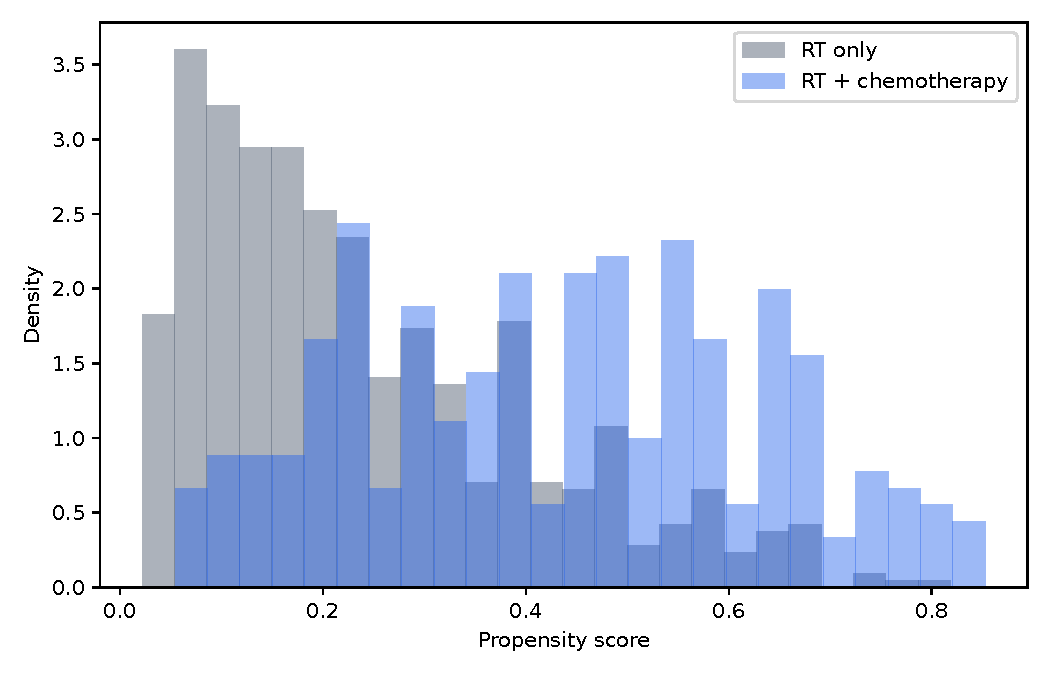
\includegraphics[width=0.76\linewidth]{figures/en/propensity_overlap.pdf}
\caption{Distribution of estimated propensity scores by observed treatment group. Density-normalized histograms compare patients receiving RT only (gray) with those receiving RT + chemotherapy (blue). The overlapping central region indicates that weighted comparisons are supported for many patients, whereas the relatively sparse group-specific tails identify limited positivity and motivate truncation of stabilized ATE weights at the 1st and 99th percentiles. ATE, average treatment effect; RT, radiotherapy.}\label{fig:1}
\end{figure}

\begin{figure}[H]
\centering
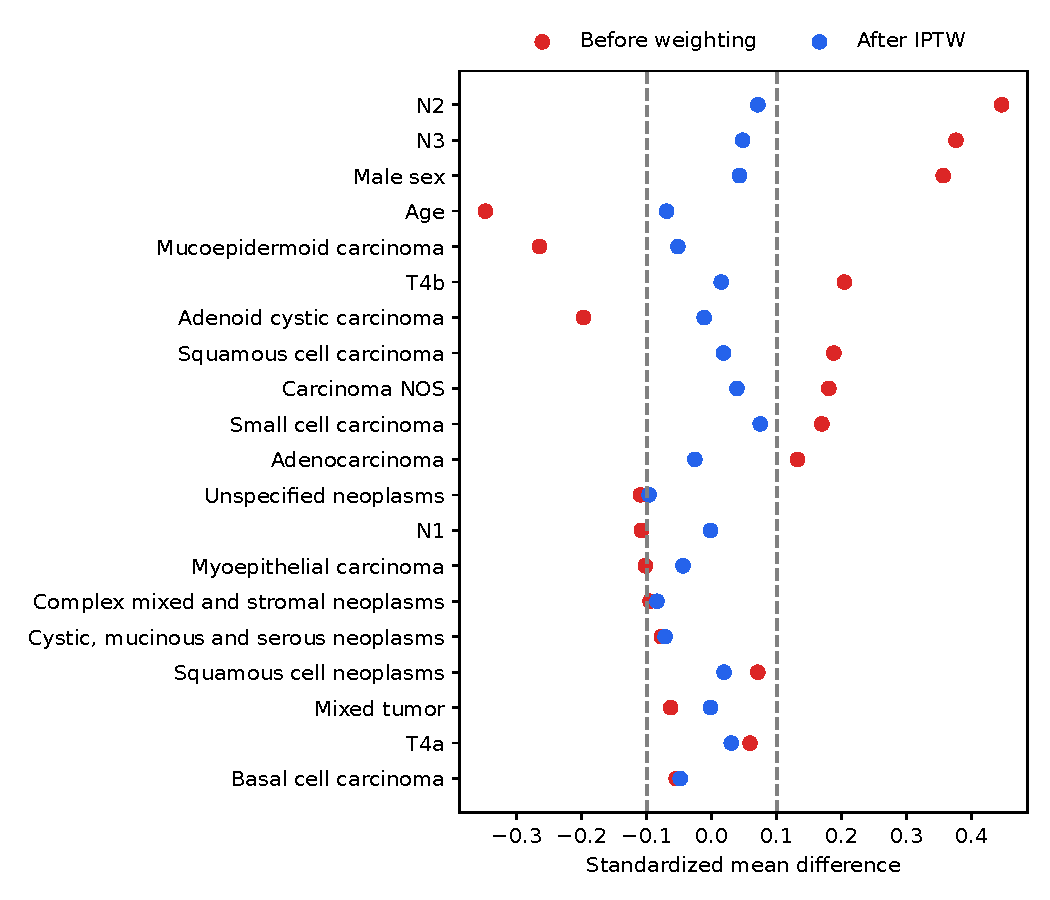
\includegraphics[width=0.68\linewidth]{figures/en/covariate_balance_love_plot.pdf}
\caption{Covariate balance before and after inverse-probability-of-treatment weighting. Points are standardized mean differences comparing RT + chemotherapy with RT only before weighting (red) and after stabilized, truncated ATE weighting (blue); the 20 encoded covariate categories with the largest absolute imbalance before weighting are displayed. The vertical dashed lines mark the prespecified |SMD| = 0.10 balance threshold; values closer to zero indicate better balance. Weighting moved nearly all measured covariates within the target range, with a maximum residual |SMD| of 0.108 in a sparse histology category. ATE, average treatment effect; IPTW, inverse-probability-of-treatment weighting; RT, radiotherapy; SMD, standardized mean difference.}\label{fig:2}
\end{figure}

\subsection{Primary effect estimate}

\begin{table}[H]
\caption{Standardized overall-survival estimates and treatment contrasts in the eligible population.}\label{tab:2}
\begin{sgatable}
\begin{tabularx}{\linewidth}{|>{\hsize=1.353\hsize}L|>{\hsize=0.647\hsize}C|>{\hsize=0.706\hsize}C|>{\hsize=1.941\hsize}C|>{\hsize=0.353\hsize}C|}
\hline
\rowcolor{sgaheader}\sgahead{Estimand} & \sgahead{RT only} & \sgahead{RT + chemotherapy} & \sgahead{Difference (RT + chemotherapy − RT only)} & \sgahead{P value} \\ \hline
RMST through 120 months & 67.1 months & 64.8 months & −2.3 months (95\% CI −9.6 to +6.0) & 0.580 \\ \hline
Survival at 60 months & — & — & −2.2 percentage points & 0.581 \\ \hline
Survival at 120 months & — & — & −2.2 percentage points & 0.578 \\ \hline
\end{tabularx}
\end{sgatable}
\tablenote{RMST values are areas under the adjusted marginal overall-survival curves through 120 months. Differences are defined as RT + chemotherapy minus RT only, so negative values favor RT only. The RMST confidence interval is the percentile interval from 1,000 patient-level bootstrap samples; two-sided P values use the bootstrap standard error. Dashes indicate that arm-specific fixed-time survival estimates are not displayed in this summary table. CI, confidence interval; RMST, restricted mean survival time; RT, radiotherapy.}
\end{table}

The standardized RMST point estimate and both fixed-time contrasts favored RT only, although none reached statistical significance. The results therefore predict no average survival benefit from chemotherapy, while the confidence interval quantifies the remaining uncertainty (Table 2). The adjusted marginal survival curves remained close throughout follow-up, with no sustained separation favoring chemotherapy (Figure 3). Consistent with this uncertainty, the patient-level bootstrap distribution of the RMST contrast was centered below zero but spanned values favoring either treatment strategy (Figure 4).

\begin{figure}[H]
\centering
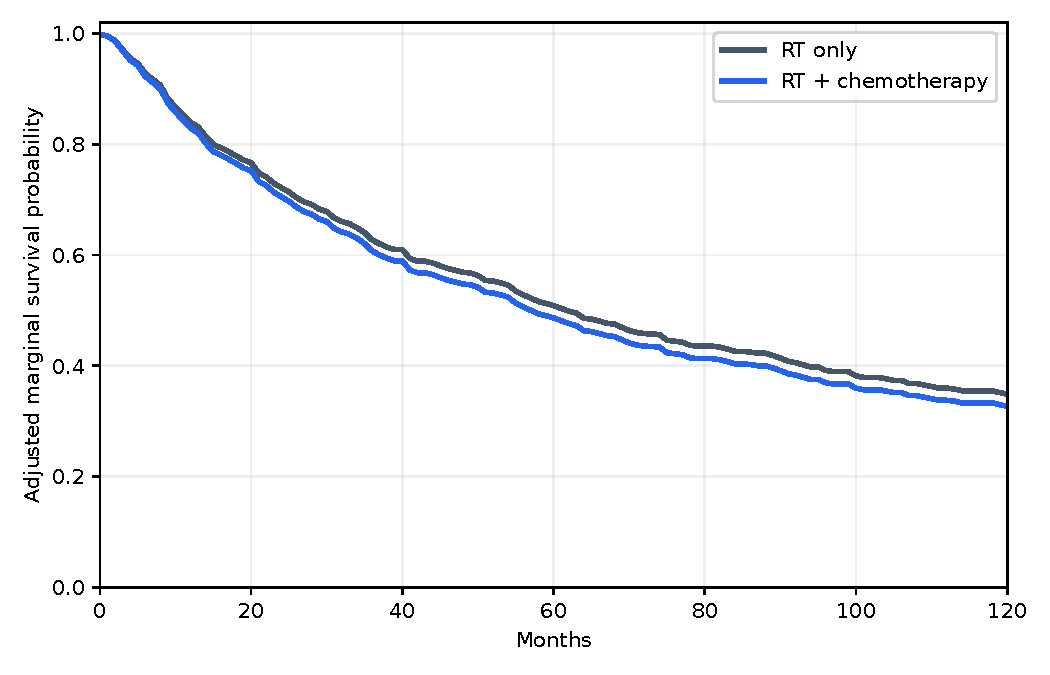
\includegraphics[width=0.76\linewidth]{figures/en/adjusted_marginal_survival.pdf}
\caption{Adjusted marginal overall-survival curves under RT only and RT + chemotherapy. For each treatment strategy, the weighted Cox model predicted every patient's counterfactual survival curve and predictions were averaged over the same 954-person eligible population. Survival was administratively truncated at 120 months. The curves remain close throughout follow-up and show no sustained separation favoring chemotherapy; their integrated areas yield 10-year RMST values of 67.1 and 64.8 months, respectively. RMST, restricted mean survival time; RT, radiotherapy.}\label{fig:3}
\end{figure}

\begin{figure}[H]
\centering
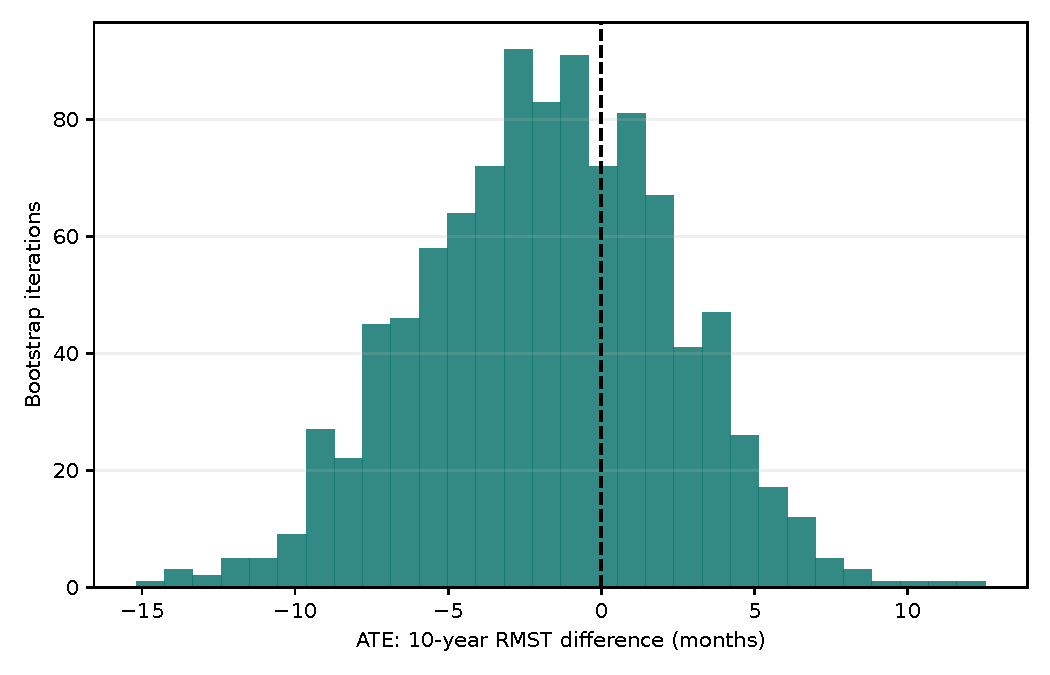
\includegraphics[width=0.76\linewidth]{figures/en/bootstrap_rmst_difference.pdf}
\caption{Patient-level bootstrap distribution of the adjusted 10-year RMST treatment contrast. Each of 1,000 iterations resampled patients and repeated cohort construction, propensity-score estimation, weight calculation and truncation, outcome-model fitting, standardization, and RMST integration. The horizontal axis is RT + chemotherapy minus RT only in months; values below zero favor RT only and values above zero favor RT + chemotherapy. The dashed vertical line marks the null value of zero. The distribution is centered at −2.3 months and crosses zero (95\% percentile CI, −9.6 to +6.0), indicating substantial uncertainty around the point estimate. ATE, average treatment effect; CI, confidence interval; RMST, restricted mean survival time; RT, radiotherapy.}\label{fig:4}
\end{figure}

\subsection{Model performance}

\begin{table}[H]
\caption{Five-fold cross-validated discrimination, prediction error, and calibration of the survival model.}\label{tab:3}
\begin{sgatable}
\begin{tabularx}{\linewidth}{|>{\hsize=2.294\hsize}L|>{\hsize=0.353\hsize}C|>{\hsize=0.353\hsize}C|}
\hline
\rowcolor{sgaheader}\sgahead{Metric} & \sgahead{5 years} & \sgahead{10 years} \\ \hline
IPCW Brier score, cross-validated mean & 0.215 & 0.188 \\ \hline
Calibration error, cross-validated mean & +0.010 & +0.013 \\ \hline
\end{tabularx}
\end{sgatable}
\tablenote{Values are means across the five held-out folds. Lower IPCW Brier scores indicate better overall prediction accuracy. Calibration error is mean predicted risk minus Kaplan–Meier observed risk, so positive values indicate slight average overprediction of mortality. The cross-validated Harrell C-index, which summarizes discrimination across follow-up rather than at a single horizon, was 0.641. IPCW, inverse probability of censoring weighting.}
\end{table}

The survival model showed moderate discrimination and acceptable prediction error at both clinical horizons. Calibration error was close to zero at 5 and 10 years, indicating little average over- or underprediction (Table 3). Performance is reported for the survival model itself; no classifier AUC is used as survival-model validation.

\subsection{Sensitivity analyses}

\begin{table}[H]
\caption{Prespecified sensitivity analyses of the adjusted treatment-effect estimate under alternative histologic eligibility definitions.}\label{tab:4}
\begin{sgatable}
\begin{tabularx}{\linewidth}{|>{\hsize=1.938\hsize}L|>{\hsize=0.363\hsize}C|>{\hsize=0.666\hsize}C|>{\hsize=0.999\hsize}C|>{\hsize=1.033\hsize}C|}
\hline
\rowcolor{sgaheader}\sgahead{Analysis} & \sgahead{N} & \sgahead{RMST difference} & \sgahead{Survival difference at 5 years} & \sgahead{Survival difference at 10 years} \\ \hline
Primary & 954 & −2.3 months & −2.2 pp & −2.2 pp \\ \hline
Excluding squamous carcinoma & 727 & −4.1 months & −3.9 pp & −4.0 pp \\ \hline
RTOG 1008-comparable histologies & 622 & −5.4 months & −5.2 pp & −5.4 pp \\ \hline
\end{tabularx}
\end{sgatable}
\tablenote{Differences are defined as RT + chemotherapy minus RT only; negative values favor RT only. Each sensitivity analysis repeated propensity-score weighting, weighted outcome modeling, and standardization within the specified cohort. The RTOG 1008-comparable subset included mucoepidermoid, adenocarcinoma, acinar cell, adenoid cystic, carcinoma NOS, and carcinoma ex pleomorphic adenoma. These analyses assess robustness to histologic eligibility and are not randomized subgroup comparisons. NOS, not otherwise specified; pp, percentage points; RMST, restricted mean survival time; RT, radiotherapy.}
\end{table}

The direction of the primary estimate persisted after excluding squamous carcinoma and after restricting the cohort to histologies comparable with RTOG 1008 (Table 4). Descriptive histology-specific estimates were unstable, including a large negative estimate for adenoid cystic carcinoma based on only 27 exposed patients, and were not interpreted as validated treatment-benefit categories. The adjusted treatment hazard ratio was 1.08 (95\% CI 0.85–1.37; robust Wald P=0.548); its point-estimate E-value was 1.36, while the confidence-interval E-value was 1.00 because the interval included the null.

The separate cancer-specific cause-specific model estimated a 10-year RMST difference of −3.7 months. It is secondary and does not replace the overall-survival endpoint.

\subsection{Illustrative N=252 simulations}

Across 1,000 secondary simulations, the mean RMST difference was −2.4 months, with individual simulated estimates ranging from −10.6 to +7.9 months. The average maximum absolute SMD across age, sex, T4, and nodal status was 0.185, demonstrating why a single random sample can appear imbalanced. These simulations are illustrative and are not the primary result.

\FloatBarrier
\section{Discussion}

In this RTOG 1008-like analysis of advanced T3/T4 salivary gland cancer, the model predicted no average overall-survival benefit from adding chemotherapy to radiotherapy. After adjustment for censoring and measured treatment-selection differences, the 10-year RMST difference was −2.3 months (95\% bootstrap CI, −9.6 to +6.0; P=0.580), and the absolute survival differences at 5 and 10 years were both −2.2 percentage points. The direction and magnitude of these estimates argue against a substantial population-wide benefit from chemotherapy intensification. This prediction is consistent with the current guideline position: postoperative radiotherapy is established for adverse features, whereas routine concurrent chemotherapy remains unsupported outside a clinical trial [1,2]. RTOG 1008 exists precisely because prospective efficacy evidence has been lacking [22–24].

The first anchor for interpretation is the postoperative radiotherapy literature. Terhaard et al. identified T3/T4 disease and incomplete resection as adverse factors for recurrence and showed that T and N stage, high grade, and perineural invasion were associated with distant metastasis and survival [4]. Mahmood et al. associated adjuvant radiotherapy with improved survival in high-grade and locally advanced major salivary gland tumors [6]. Schoenfeld et al. reported that postoperative intensity-modulated radiotherapy was well tolerated and achieved high local control [7], while Hosni et al. emphasized that distant metastasis remained a dominant pattern of failure in high-risk patients despite postoperative radiotherapy [8]. The contemporary systematic review by Wang et al. likewise supported the locoregional role of postoperative radiotherapy while underscoring the absence of strong global evidence for adding concurrent chemotherapy [9]. Parotid- and histology-specific series further reinforce the use of postoperative radiotherapy for adverse features such as positive margins, high grade, and T3/T4 disease [25–27]. Taken together, these studies establish radiotherapy as the locoregional backbone of treatment but do not establish that chemotherapy adds a survival benefit.

The second and more direct anchor is the comparative chemoradiotherapy literature. Early institutional series suggested that concurrent chemotherapy might improve outcomes in selected high-risk patients [11,12]. These reports provided an important biological and clinical rationale for treatment intensification, but their small sample sizes, nonrandomized designs, and susceptibility to treatment-selection bias limited causal interpretation. Subsequent institutional comparisons did not demonstrate a clear overall-survival advantage for chemoradiotherapy [13,16]. In older patients, the SEER-Medicare analysis by Tanvetyanon et al. reported outcomes that did not favor chemotherapy intensification [14], and the large NCDB analysis by Amini et al. found no overall-survival advantage for adjuvant chemoradiotherapy over radiotherapy alone [15]. These larger datasets shifted the balance of evidence away from routine chemotherapy use, although residual confounding remained unavoidable.

More recent studies have largely followed the same direction while suggesting that any benefit may be concentrated in selected biological or clinicopathologic subsets. Kang et al. found no overall- or disease-specific-survival benefit from adding chemotherapy in advanced major salivary gland cancer [19]. Hsieh et al. and Shen et al., however, described possible signals in patients with nodal disease, R2 resection, adenoid cystic carcinoma, or combinations of T3/T4 high-grade tumors and heavy nodal burden [20,21]. Similarly, the propensity-matched adenoid cystic carcinoma study by Hsieh et al. suggested improved locoregional control without a corresponding overall-survival improvement [17]. This distinction is clinically important: a radiosensitizing effect may improve local control without overcoming distant metastatic risk or translating into longer survival. The available evidence therefore does not support the routine addition of chemotherapy across an unselected high-risk population, but it also does not exclude benefit in a biologically enriched subgroup.

Our findings follow the dominant direction of the comparative evidence. The primary estimate did not favor chemotherapy, and neither exclusion of squamous carcinoma nor restriction to RTOG 1008-comparable histologies revealed a global survival advantage. The central prediction is therefore that chemotherapy will not improve average overall survival across a broad population with advanced T3/T4 disease. As in the recent retrospective literature, a benefit confined to a narrowly selected biological subgroup remains possible but unproven.

The most important prospective context is RTOG 1008. That trial was designed because the retrospective evidence was insufficient and conflicting: early small studies suggested possible benefit [11,12], whereas larger registry and institutional comparisons failed to confirm a consistent survival advantage [13–16]. RTOG 1008 directly compares postoperative radiotherapy alone with radiotherapy plus weekly cisplatin in resected high-risk malignant salivary gland tumors [22–24]. The GORTEC-REFCOR SANTAL study similarly evaluates radiotherapy with or without cisplatin in salivary gland and sinonasal tumors [28]. Together, these trials show that platinum radiosensitization remains a plausible research strategy, while ASCO and ESMO-EURACAN guidelines do not endorse its routine use outside clinical trials [1,2]. This analysis should therefore not be framed as a substitute for RTOG 1008. Its principal value is prospective falsifiability: it provides a pre-results model-based prediction that can later be compared with randomized evidence.

If RTOG 1008 demonstrates a clinically meaningful survival benefit, it will falsify the present prediction and identify dimensions of treatment effect not captured by the registry model. If it does not demonstrate benefit, the result will support the prediction that chemotherapy should not be routinely added to postoperative radiotherapy outside selected subgroups or clinical trials.

This work also highlights the distinction between prognostic and predictive modeling. Existing models estimate recurrence, postoperative survival, distant metastasis, or baseline prognosis [29–35]. High risk, however, does not automatically imply chemotherapy benefit. By estimating survival under both treatment strategies in the same population, this analysis directly targets the incremental effect of chemotherapy rather than prognosis alone. Its clinically testable prediction is straightforward: adding chemotherapy to radiotherapy will not improve average overall survival in advanced T3/T4 salivary gland cancer.

\FloatBarrier
\section{Limitations}

This registry analysis remains susceptible to residual confounding, particularly from pathologic risk factors, performance status, treatment timing, and treatment details not captured in the extract. Diagnosis was the available time origin, treatment concurrency could not be confirmed, and histology-specific estimates were sparse. The Cox model also imposes proportional hazards, and validation was internal. These limitations affect causal certainty and subgroup resolution but do not change the study's prespecified population-level prediction.

\FloatBarrier
\section{Conclusion}

The model predicts that adding chemotherapy to radiotherapy does not improve average overall survival in advanced T3/T4 salivary gland cancer. The adjusted 10-year RMST difference was −2.3 months, with no favorable effect at 5 or 10 years. This falsifiable pre-results prediction now awaits comparison with RTOG 1008.

\clearpage
\section{References}

\begin{sgareferences}
\item Geiger JL, Ismaila N, Beadle B, Caudell JJ, Chau N, Deschler D, et al. Management of Salivary Gland Malignancy: ASCO Guideline. J Clin Oncol. 2021;39:1909-1941. doi:10.1200/JCO.21.00449.
\item van Herpen C, Locati LD, But-Hadzic J, Bossi P, Cavalieri S, Licitra L, et al. Salivary gland cancer: ESMO-EURACAN Clinical Practice Guideline for diagnosis, treatment and follow-up. ESMO Open. 2022. PMID:36567082.
\item PDQ Adult Treatment Editorial Board. Salivary Gland Cancer Treatment (PDQ). National Cancer Institute; updated 2025.
\item Terhaard CHJ, Lubsen H, van der Tweel I, Hilgers FJM, Eijkenboom WMH, Marres HAM, et al. Salivary gland carcinoma: independent prognostic factors for locoregional control, distant metastases, and overall survival: results of the Dutch head and neck oncology cooperative group. Head Neck. 2004;26:681-693. PMID:15287035.
\item Mendenhall WM, Morris CG, Amdur RJ, Werning JW, Hinerman RW, Villaret DB. Radiotherapy alone or combined with surgery for salivary gland carcinoma. Cancer. 2005;103:2544-2550. PMID:15880750.
\item Mahmood U, Koshy M, Goloubeva O, Suntharalingam M. Adjuvant radiation therapy for high-grade and/or locally advanced major salivary gland tumors. Arch Otolaryngol Head Neck Surg. 2011. PMID:22006781.
\item Schoenfeld JD, Sher DJ, Norris CM Jr, Haddad RI, Posner MR, Balboni TA, et al. Salivary gland tumors treated with adjuvant intensity-modulated radiotherapy with or without concurrent chemotherapy. Int J Radiat Oncol Biol Phys. 2012;82:308-314. PMID:21075557.
\item Hosni A, Huang SH, Goldstein D, Xu W, Chan B, Hansen A, et al. Outcomes and prognostic factors for major salivary gland carcinoma following postoperative radiotherapy. Oral Oncol. 2016;54:75-80. PMID:26723908.
\item Wang J, et al. The Current Position of Postoperative Radiotherapy for Salivary Gland Cancer: A Systematic Review and Meta-Analysis. Cancers. 2024;16:2375.
\item Cerda T, Sun XS, Vignot S, et al. A rationale for chemoradiation versus radiotherapy in salivary gland cancers? Crit Rev Oncol Hematol. 2014;91:142-158. PMID:24636481.
\item Pederson AW, Salama JK, Haraf DJ, Witt ME, Stenson KM, Portugal L, et al. Adjuvant chemoradiotherapy for locoregionally advanced and high-risk salivary gland malignancies. Head Neck Oncol. 2011;3:31. PMID:21791072.
\item Tanvetyanon T, Qin D, Padhya T, McCaffrey J, Zhu W, Boulware D, et al. Outcomes of postoperative concurrent chemoradiotherapy for locally advanced major salivary gland carcinoma. Arch Otolaryngol Head Neck Surg. 2009;135:687-692. doi:10.1001/archoto.2009.70.
\item Mifsud MJ, Tanvetyanon T, McCaffrey JC, Otto KJ, Padhya TA, Kish J, et al. Adjuvant radiotherapy versus concurrent chemoradiotherapy for the management of high-risk salivary gland carcinomas. Head Neck. 2016;38:1628-1633. doi:10.1002/hed.24484.
\item Tanvetyanon T, Fisher K, Caudell J, Otto K, Padhya T, Trotti A. Adjuvant chemoradiotherapy versus radiotherapy alone for locally advanced salivary gland carcinoma among older patients. Head Neck. 2016;38:863-870. PMID:26340707.
\item Amini A, Waxweiler TV, Brower JV, Jones BL, McDermott JD, Raben D, et al. Association of adjuvant chemoradiotherapy vs radiotherapy alone with survival in patients with resected major salivary gland carcinoma: data from the National Cancer Data Base. JAMA Otolaryngol Head Neck Surg. 2016;142:1100-1110. doi:10.1001/jamaoto.2016.2168.
\item Gebhardt BJ, Ohr JP, Ferris RL, Duvvuri U, Johnson JT, Kim S, et al. Concurrent chemoradiotherapy in the adjuvant treatment of salivary gland malignancies. Am J Clin Oncol. 2018;41:888-893. PMCID:PMC6587550.
\item Hsieh CE, Lin CY, Lee LY, Yang LY, Wang CC, Wang HM, et al. Adding concurrent chemotherapy to postoperative radiotherapy improves locoregional control but not overall survival in patients with salivary gland adenoid cystic carcinoma: a propensity score matched study. Radiat Oncol. 2016;11:47. doi:10.1186/s13014-016-0617-7.
\item Yan W, Huang S, et al. Postoperative chemoradiotherapy versus radiotherapy alone for major salivary gland malignancies: a stratified study based on the external validation of the distant metastasis risk score model. Cancers. 2022;14:5583.
\item Kang NW, Kuo YH, Wu HC, Ho CH, Chen YC, Yang CC. No survival benefit from adding chemotherapy to adjuvant radiation in advanced major salivary gland cancer. Sci Rep. 2022;12:20862. doi:10.1038/s41598-022-25468-9.
\item Hsieh RCE, et al. A multicenter retrospective analysis of patients with salivary gland carcinoma receiving postoperative chemoradiotherapy versus postoperative radiotherapy. Radiother Oncol. 2023. PMID:37659659.
\item Shen Y, Shan J. Chemoradiotherapy versus radiotherapy in high risk salivary gland cancer. World J Surg Oncol. 2024;22:181. doi:10.1186/s12957-024-03456-9.
\item NRG Oncology. RTOG-1008: A randomized phase II/phase III study of adjuvant concurrent radiation and chemotherapy versus radiation alone in resected high-risk malignant salivary gland tumors. NRG Oncology protocol page.
\item NRG Oncology. RTOG 1008 protocol, version 11/5/2015. Required sample size: Phase II 120; Phase III 252.
\item ClinicalTrials.gov. Radiation Therapy With or Without Chemotherapy in Treating Patients With High-Risk Malignant Salivary Gland Tumors. Identifier: NCT01220583.
\item Kim YH, et al. Evaluation of prognostic factors for the parotid cancer treated with surgery and postoperative radiotherapy. Cancer Res Treat. 2020. PMID:31480828.
\item Park G, et al. Postoperative radiotherapy for mucoepidermoid carcinoma of major salivary glands: long-term results of a single-institution experience. Radiat Oncol J. 2018. PMID:30630270.
\item Katano A, et al. Postoperative radiotherapy for malignant major salivary gland tumors. 2023.
\item GORTEC/REFCOR. Treatment of Salivary Glands and Nasal Tumors (SANTAL). ClinicalTrials.gov Identifier: NCT02998385.
\item Lukovic J, Sultana R, et al. Development and validation of a clinical prediction-score model for distant metastases in salivary gland cancer. Oral Oncol. 2020. PMID:31959347.
\item Ali S, Palmer FL, Yu C, DiLorenzo M, Shah JP, Kattan MW, et al. A predictive nomogram for recurrence of carcinoma of the major salivary glands. JAMA Otolaryngol Head Neck Surg. 2013;139:698-705. doi:10.1001/jamaoto.2013.3347.
\item Ali S, Palmer FL, Yu C, DiLorenzo M, Shah JP, Kattan MW, Patel SG, Ganly I. Postoperative nomograms predictive of survival after surgical management of malignant tumors of the major salivary glands. Ann Surg Oncol. 2014;21:637-642. PMID:24132626.
\item Hay A, Migliacci J, Karassawa Zanoni D, et al. Validation of nomograms for overall survival, cancer-specific survival and recurrence in major salivary gland cancer. Head Neck. 2018. PMID:29389040.
\item Chen Y, Li Y, et al. Prognostic risk factor of major salivary gland carcinomas and survival prediction model based on random survival forests. Cancer Med. 2023. PMID:36934429.
\item Du W, et al. Prognostic prediction model for salivary gland carcinoma based on machine learning. 2024. PMID:38981745.
\item Jacobs CD, et al. Prediction model to estimate overall survival benefit of postoperative radiation therapy for resected major salivary gland cancers. Oral Oncol. 2022. doi:10.1016/j.oraloncology.2022.105902.
\end{sgareferences}

\clearpage
\section{Supplementary Material}

\begin{table}[H]
\renewcommand\thetable{S\arabic{table}}\setcounter{table}{0}
\caption{Cohort selection from the standardized SEER-derived extract.}\label{tab:S1}
\begin{sgatable}
\begin{tabularx}{\linewidth}{|>{\hsize=1.707\hsize}L|>{\hsize=0.632\hsize}C|>{\hsize=0.661\hsize}C|}
\hline
\rowcolor{sgaheader}\sgahead{Selection step} & \sgahead{Remaining, n} & \sgahead{Excluded at step, n} \\ \hline
Source standardized records & 4,657 & 0 \\ \hline
T3/T4 disease & 1,667 & 2,990 \\ \hline
Known N category & 1,391 & 276 \\ \hline
Radiotherapy recorded & 954 & 437 \\ \hline
Nonmissing survival time & 954 & 0 \\ \hline
\end{tabularx}
\end{sgatable}
\tablenote{Criteria were applied sequentially. Surgery, postoperative intent of radiotherapy, M stage, and diagnosis year are not available in the extract and could not be used as eligibility criteria. SEER, Surveillance, Epidemiology, and End Results.}
\end{table}

\end{document}
